% !TeX root = ../Thesis.tex

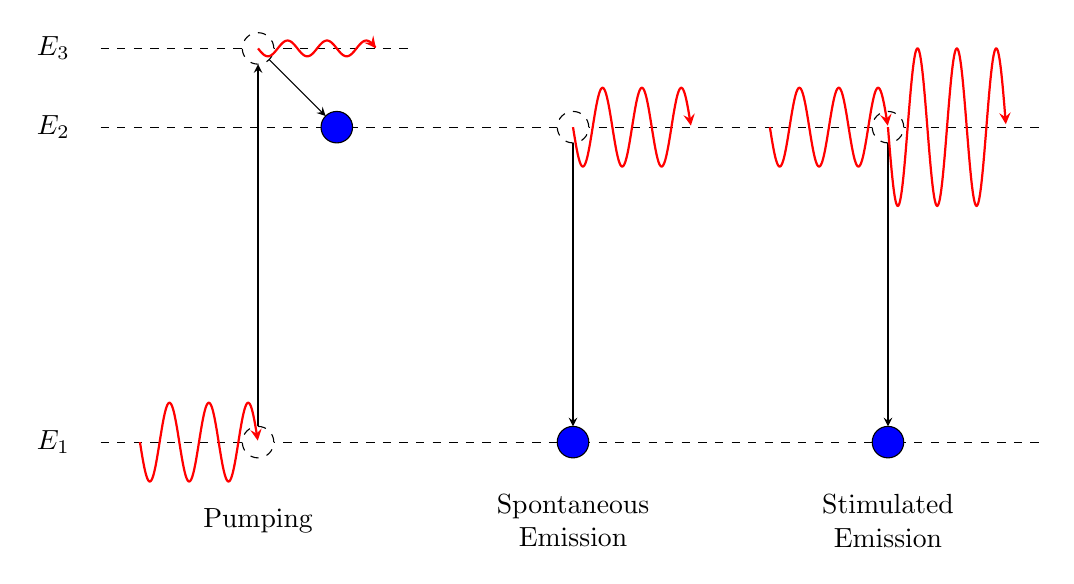
\begin{tikzpicture}
% Energy levels
\draw [dashed] (0,0) -- (12,0) node [pos = -0.05] {$E_1$};
\draw [dashed] (0,4) -- (12,4) node [pos = -0.05] {$E_2$};
\draw [dashed] (0,5) -- (4,5) node [pos = -0.15] {$E_3$};

% Transition arrows
\draw[->, >=stealth] (2,0.2) -- (2,4.8);
\draw[->, >=stealth] (2,5) -- (3-0.2*0.707,4+0.2*0.707);
\draw[<-, >=stealth] (6,0.2) -- (6,4);
\draw[<-, >=stealth] (10,0.2) -- (10,4);

% Circles
% Bottom
\filldraw[fill=white, draw=black, dashed] (2,0) circle (0.2);
\filldraw[fill=blue, draw=black] (6,0) circle (0.2);
\filldraw[fill=blue, draw=black] (10,0) circle (0.2);
% Top
\filldraw[fill=white, draw=black, dashed] (2,5) circle (0.2);
\filldraw[fill=blue, draw=black] (3,4) circle (0.2);
\filldraw[fill=white, draw=black, dashed] (6,4) circle (0.2);
\filldraw[fill=white, draw=black, dashed] (10,4) circle (0.2);

% Photons
\draw [domain=0.5:2, samples=250, red, thick, ->, >=stealth] plot (\x, {-0.5*sin(4*pi*deg(\x-2))});
\draw [domain=2:3.5, samples=250, red, thick, ->, >=stealth] plot (\x, {5-0.1*sin(4*pi*deg(\x-2))});
\draw [domain=6:7.5, samples=250, red, thick, ->, >=stealth] plot (\x, {4-0.5*sin(4*pi*deg(\x-6))});
\draw [domain=8.5:10, samples=250, red, thick, ->, >=stealth] plot (\x, {4-0.5*sin(4*pi*deg(\x-10))});
\draw [domain=10:11.5, samples=250, red, thick, ->, >=stealth] plot (\x, {4-sin(4*pi*deg(\x-10))});

% Labels
\node at (2, -1){Pumping};
\node [align=center] at (6, -1){Spontaneous \\ Emission};
\node [align=center] at (10, -1){Stimulated \\ Emission};
\end{tikzpicture}